\chapter{Bayesian network lab}
\label{cha:bay_net_lab}

Let's now consider a simple classifier that can be used to exploit a BN.\\

\section{Naive bayes}
We are facing the problem of classification. BN try to model the domain with variables and relationship that make sense of the data. 
When we have a set of input and an output to be computed (standard setting for supervised learning) starting from the knowledge. 
In plain classification we know that a set of known variables in input $\Vec{x}$ and a target $y$ with no ambiguity.\\
The idea of naive bayes classifier is a probabilistic algorithm for classification. We decide we want to compute the argmax given the data. 
$$y* = argmax_{y \in Y} P(y|\Vec{x}) = argmax _{y \in Y} \frac{P(\Vec{x}|y)P(y)}{P(\Vec{x})}$$
but since $P(\Vec{x})$ is constant (given) then we can simply consider 
$$y* = argmax_{y \in Y} {P(\Vec{x}|y)P(y)}$$
Now, here we are not able to model $P(\Vec{x}|y)$ the joint probability (when $\Vec{x}$ increases dramatically in dimension). 
$$P(\Vec{x}|y) = P(x_1, \dots, x_n| y) P(y)$$
When everything is binary I get $2^n$ configuration to be modelled, which is pretty complex. I would need tons of data in order to learn every configuration. This is not always feasible.\\

We consider a simplification as assumption: \textbf{a naive bayes assumes that the different features ($x_1, \dots, x_n$) of the input are independent given the class}. This means that I can simplify the probability into: 
$$P(y|\Vec{x}) = \prod_{i=1}^n P(x_i|y)P(y)$$
with $n$ number of features. 
This is rather simple because we consider separate table for each features, therefore we can estimate parameters locally and this allows to have much less parameters. This classifier is not always accurate (it is indeed naive) but it is a good starting point.
The bayesian network will look like this: \\
\begin{figure}[ht]
    \centering
    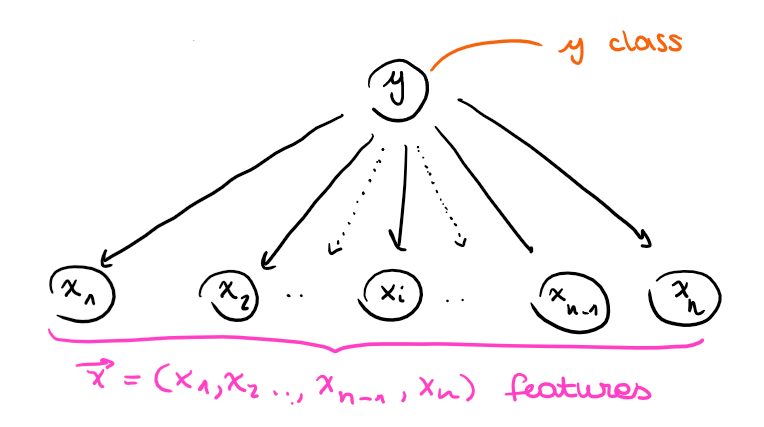
\includegraphics[scale=0.4]{images/naiive.png}
    \caption{basic representation of a naive NB}
    \label{fig:naive}
\end{figure}
where we have a connection from the class $y$ to each of the features $x_1, \dots, x_n$ but features are not connected to each other.

    \subsection{Text classification}
    Let' consider having a piece of text $x$ and we consider words as features
    $$\Vec{x} = (w_1, \dots, w_n)$$
    The naive bayes assumption says that the probability of finding a word or another is the same (so the probabilities are independent). The piece of text is turned into a \textit{bag of words}, therefore we forget about the position.\\
    This is a simplifying assumption because words that are often associated together (machine + learning, artificial + intelligence ...) are learned independently but as a matter of fact they are not.
    The way to model a naive bayes classifier is by saying that each word is modelled as independent items belonging to a greater set of words $\mathcal{V}$ (as vocabulary). 
    Each word can take a number of values corresponding at most with the size of the vocabulary.
    The naive classifier will be
    $$\prod_{i=1}^{|\Vec{x}|} P(w_i|y)P(y)$$
    This is a multinomial distribution that is specific for every types of topic $y$ (biology, machine learning, mathematics, physics...) so we can get all possible words for all possible class. 
    \begin{figure}[ht]
        \centering
        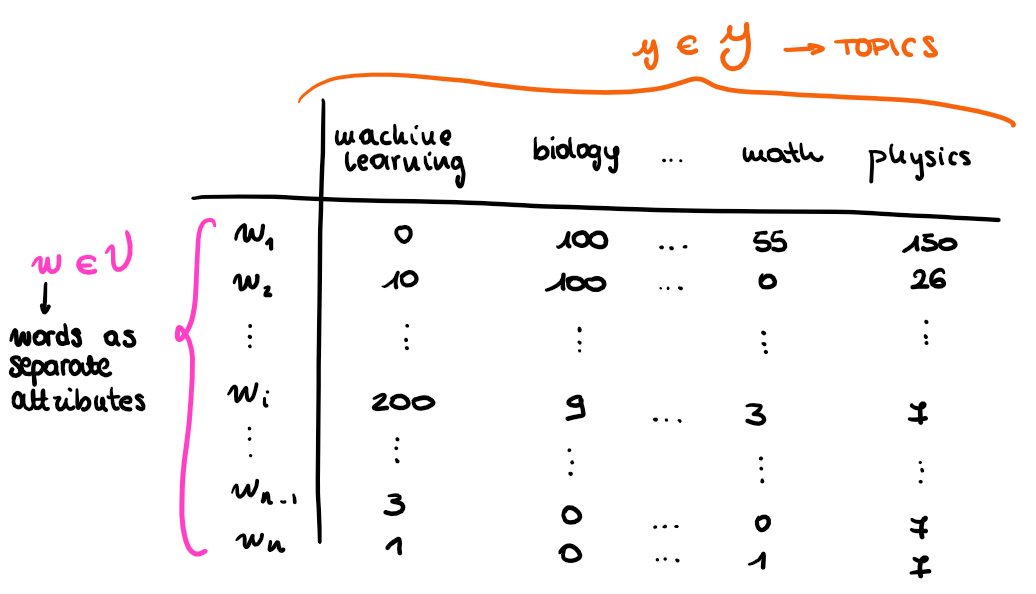
\includegraphics[scale=0.4]{images/text classification.png}
        \caption{Example of recurrences of each word in the vocabulary for each class (topic) as independent variables}
        \label{fig:naive_text}
    \end{figure}
    Each column is a multinomial distribution over size of $|\mathcal{V}|$ possible values. In this way the different elements in the product are modelled in the same distribution. Typically we have multiple times the same word in the document.
    The naive bayes assumption can not always be applied as we have seen so far since in some cases the dataset is made as separate attributes (height, weight, hair color...) and need to be modelled with different models (continuous/discrete values).